\begin{PROBLEM}
    \p
دنباله‌ای با دامنه‌ی نامحدود از اشکال زیر وجود دارد. این چهار شکل، به ترتیب از چپ به راست، چهار عضو اول این دنباله هستند.‌
	 $a_i$
	را معادل تعداد دایره‌های موجود در عضو 
$i$-ام این دنباله در نظر بگیرید.
	جمله‌ی عمومی دنباله $a_i$ را بر حسب
	$n$
	به‌دست آورید.
	\p
	\begin{center}
		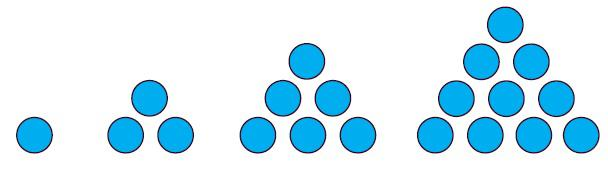
\includegraphics[scale=0.3]{./1.jpg}
	\end{center}
    \SOLUTION{
        \p
       هر شکل نسبت به شکل قبلی یک ردیف بیشتر دارد یعنی: 
    		$$a_1 = 1$$
    		$$a_2 = a_1 + 2$$
    		$$a_3 = a_2 + 3$$
    		$$\vdots$$
			$$a_n = a_{n-1} + n$$
			\begin{center}
				$\rule{0.4\textwidth}{0.8pt}$
				\Huge{+}
			\end{center}
            $$a_1 + a_2 + ... + a_n = a_1 + a_2 + ... + a_{n-1} + 1 + 2 + ... + n$$
            $$a_n = 1 + 2 + 3 + ... + n = \frac{n(n+1)}{2}$$
        }
\end{PROBLEM}